\documentclass[11pt, letterpaper, titlepage]{article}
\usepackage[utf8]{inputenc}
\usepackage{geometry}
\usepackage{color,graphicx,overpic} 
\usepackage{fancyhdr}
\usepackage{amsmath,amsthm,amsfonts,amssymb}
\usepackage{mathtools}
\usepackage{hyperref}
\usepackage{multicol}
\usepackage{array}
\usepackage{float}
\usepackage{blindtext}
\usepackage{longtable}
\usepackage{scrextend}
\usepackage[font=small,labelfont=bf]{caption}
\usepackage[framemethod=tikz]{mdframed}
\usepackage{calc}
\usepackage{titlesec}
\usepackage{listings}
\usepackage[normalem]{ulem}
\usepackage{tabularx}
\usepackage{mathrsfs}
\usepackage{bookmark}
\usepackage{apple_emoji}
\usepackage{setspace}
\usepackage{ragged2e}
\usepackage{ltablex}
\usepackage{xurl}
\usepackage{siunitx}
\usepackage{lastpage}
\usepackage{enumitem}
\usepackage{minted}
\usepackage{paracol}
\usepackage{booktabs}

\setlist{topsep=0pt}
\mathtoolsset{showonlyrefs}  
\usetikzlibrary{arrows.meta}
\allowdisplaybreaks

\DeclarePairedDelimiter\ceil{\lceil}{\rceil}
\DeclarePairedDelimiter\floor{\lfloor}{\rfloor}
\DeclarePairedDelimiter\bracks{\left(}{\right)}

\newcolumntype{b}{X}
\newcolumntype{s}{>{\hsize=.5\hsize}X}
\newcolumntype{P}[1]{>{\centering\arraybackslash}p{#1}}

\definecolor{bg}{rgb}{0.95,0.95,0.95}

\usemintedstyle{tango}
\setminted{linenos}
\setmintedinline{bgcolor=bg,style=bw}

\tikzset{minimum size=0.75cm}

\geometry{top=2.54cm, left=2.54cm, right=2.54cm, bottom=2.54cm}
\setlength{\headheight}{20pt}
\setlength{\parskip}{0.5cm}
\setlength{\parindent}{0cm}

\newcommand{\B}{\includegraphics[height=1.5em, valign=B, raise=-0.2em]{BigB.png}} 
\newcommand{\textbr}[1]{\textbf{\color{red}{#1}}}

\pagestyle{fancy}
\fancyhf{}
\rhead{\B enjamin Kong | 1573684}
\lhead{\textit{CMPUT 204 Assignment 8 🚗 🚕 🚙}}
\rfoot{Page \thepage\ of\ \pageref{LastPage}}

\begin{document}
\onehalfspacing

\subsection*{Problem 1.}
\begin{enumerate}[label=(\alph*)]
    \item The BFS tree is shown below.
    \begin{figure}[H]
        \centering
        \caption{BFS tree.}
        \begin{tikzpicture}[
            level/.style={sibling distance=25mm}, 
            edge from parent/.style={draw,-{Latex[width=2mm]}}
            ]
            \node[circle,draw] at (0,0) {A}
                child{node[circle,draw] {B}
                    child{node[circle,draw] {C}
                        child{node[circle,draw] {G}
                            child{node[circle,draw] {F}}
                            child[missing] {}
                        }
                        child[missing] {}
                    }
                    child[missing] {}
                }
                child[missing] {};
            \node[circle,draw] at (2,-3) {D};
            \node[circle,draw] at (6,-3) {E};
        \end{tikzpicture}
    \end{figure}
    The classification of each edge is given below.
    \begin{tabularx}{\textwidth}{cc}
        \caption{Classification of each edge for the BFS tree.} \\
        \toprule
        \textbf{Edge} & \textbf{Classification} \\
        \midrule()
        (A, B) & Tree edge \\
        (B, C) & Tree edge \\
        (C, A) & Back edge \\
        (C, G) & Tree edge \\
        (D, A) & Cross edge \\
        (D, C) & Cross edge \\
        (D, F) & Cross edge \\
        (E, B) & Cross edge \\
        (E, C) & Cross edge \\
        (E, G) & Cross edge \\
        (F, C) & Back edge \\
        (G, F) & Tree edge \\
        \bottomrule
    \end{tabularx}

    \newpage
    
    The DFS tree is shown below.
    \begin{figure}[H]
        \centering
        \caption{DFS tree.}
        \begin{tikzpicture}[
            level/.style={sibling distance=25mm}, 
            edge from parent/.style={draw,-{Latex[width=2mm]}}
            ]
            \node[circle,draw,label={[]right:[1, 10]}] at (0,0) {A}
                child{node[circle,draw,label={[]right:[2, 9]}] {B}
                    child{node[circle,draw,label={[]right:[3, 8]}] {C}
                        child{node[circle,draw,label={[]right:[4, 7]}] {G}
                            child{node[circle,draw,label={[]right:[5, 6]}] {F}}
                            child[missing] {}
                        }
                        child[missing] {}
                    }
                    child[missing] {}
                }
                child[missing] {};
            \node[circle,draw,label={[]right:[11, 12]}] at (2,-3) {D};
            \node[circle,draw,label={[]right:[13, 14]}] at (6,-3) {E};
        \end{tikzpicture}
    \end{figure}
    The classification of each edge is given below.
    \begin{tabularx}{\textwidth}{cc}
        \caption{Classification of each edge for the DFS tree.} \\
        \toprule
        \textbf{Edge} & \textbf{Classification} \\
        \midrule()
        (A, B) & Tree edge \\
        (B, C) & Tree edge \\
        (C, A) & Back edge \\
        (C, G) & Tree edge \\
        (D, A) & Cross edge \\
        (D, C) & Cross edge \\
        (D, F) & Cross edge \\
        (E, B) & Cross edge \\
        (E, C) & Cross edge \\
        (E, G) & Cross edge \\
        (F, C) & Back edge \\
        (G, F) & Tree edge \\
        \bottomrule
    \end{tabularx}

    \newpage

    \item The BFS tree is shown below.
    \begin{figure}[H]
        \centering
        \caption{BFS tree.}
        \begin{tikzpicture}[
            level/.style={sibling distance=25mm}, 
            edge from parent/.style={draw,-{Latex[width=2mm]}}
            ]
            \node[circle,draw] {A}
                child{node[circle,draw] {B}
                    child{node[circle,draw] {E}}
                    child[missing] {}
                }
                child{node[circle,draw] {C}}
                child{node[circle,draw] {D}
                    child{node[circle,draw] {F}
                        child{node[circle,draw] {G}}
                        child[missing] {}
                    }
                    child{node[circle,draw] {H}}
                };
        \end{tikzpicture}
    \end{figure}
    The classification of each edge is given below.
    \begin{tabularx}{\textwidth}{cc}
        \caption{Classification of each edge for the BFS tree.} \\
        \toprule
        \textbf{Edge} & \textbf{Classification} \\
        \midrule()
        (A, B) & Tree edge \\
        (A, C) & Tree edge \\
        (A, D) & Tree edge \\
        (B, E) & Tree edge \\
        (C, D) & Cross edge \\
        (D, F) & Tree edge \\
        (D, H) & Tree edge \\
        (E, A) & Back edge \\
        (E, C) & Cross edge \\
        (F, G) & Tree edge \\
        (G, D) & Back edge \\
        (H, C) & Cross edge \\
        (H, G) & Cross edge \\
        \bottomrule
    \end{tabularx}

    \newpage
    
    The DFS tree is shown below.
    \begin{figure}[H]
        \centering
        \caption{DFS tree.}
        \begin{tikzpicture}[
            level/.style={sibling distance=25mm}, 
            edge from parent/.style={draw,-{Latex[width=2mm]}}
            ]
            \node[circle,draw,label={[]right:[1, 16]}] {A}
                child{node[circle,draw,label={[]right:[2, 15]}] {B}
                    child{node[circle,draw,label={[]right:[3, 14]}] {E}
                        child{node[circle,draw,label={[]right:[4, 13]}] {C}
                            child{node[circle,draw,label={[]right:[5, 12]}] {D}
                                child{node[circle,draw,label={[]right:[6, 9]}] {F}
                                    child{node[circle,draw,label={[]right:[7, 8]}] {G}}
                                    child[missing] {}
                                }
                                child{node[circle,draw,label={[]right:[10, 11]}] {H}}
                            }
                            child[missing] {}
                        }
                        child[missing] {}
                    }
                    child[missing] {}
                }
                child[missing] {};
        \end{tikzpicture}
    \end{figure}
    The classification of each edge is given below.
    \begin{tabularx}{\textwidth}{cc}
        \caption{Classification of each edge for the DFS tree.} \\
        \toprule
        \textbf{Edge} & \textbf{Classification} \\
        \midrule()
        (A, B) & Tree edge \\
        (A, C) & Forward edge \\
        (A, D) & Forward edge \\
        (B, E) & Tree edge \\
        (C, D) & Tree edge \\
        (D, F) & Tree edge \\
        (D, H) & Tree edge \\
        (E, A) & Back edge \\
        (E, C) & Tree edge \\
        (F, G) & Tree edge \\
        (G, D) & Back edge \\
        (H, C) & Back edge \\
        (H, G) & Cross edge \\
        \bottomrule
    \end{tabularx}
\end{enumerate}

\newpage

\subsection*{Problem 2.}
\begin{enumerate}[label=(\alph*)]
    \item The DFS tree of $G^T$ produced by traversing nodes in decreasing $ftime$ is shown below.
    \begin{figure}[H]
        \centering
        \caption{DFS tree of $G^T$ produced by traversing nodes in decreasing $ftime$.}
        \begin{tikzpicture}[
            level/.style={sibling distance=25mm}, 
            edge from parent/.style={draw,-{Latex[width=2mm]}}
            ]
            \node[circle,draw,label={[]right:[5, 14]}] at (0,0) {A}
                child{node[circle,draw,label={[]right:[6, 13]}] {C}
                    child{node[circle,draw,label={[]right:[7, 8]}] {B}}
                    child{node[circle,draw,label={[]right:[9, 12]}] {F}
                        child{node[circle,draw,label={[]right:[10, 11]}] {G}}
                        child[missing] {}
                    }
                }
                child[missing] {};
            \node[circle,draw,label={[]right:[3, 4]}] at (4,-3) {D};
            \node[circle,draw,label={[]right:[1, 2]}] at (8,-3) {E};
        \end{tikzpicture}
    \end{figure}
    The component graph illustrating the SCCs is shown below.
    \begin{figure}[H]
        \centering
        \caption{Component graph illustrating the SCCs.}
        \begin{tikzpicture}
            \node[circle,minimum size= 1.8cm,draw] (A) at (0,0) {E};
            \node[circle,minimum size= 1.8cm,draw] (B) at (3,0) {ABCFG};
            \node[circle,minimum size= 1.8cm,draw] (C) at (6,0) {D};
            
            \draw[-{Latex[width=2mm]}] (A) -- (B);
            \draw[-{Latex[width=2mm]}] (C) -- (B);
        \end{tikzpicture}
    \end{figure}
    A topological sorting of the component graph is E, D, ABCFG.

    \newpage

    \item The DFS tree of $G^T$ produced by traversing nodes in decreasing $ftime$ is shown below.
    \begin{figure}[H]
        \centering
        \caption{DFS tree of $G^T$ produced by traversing nodes in decreasing $ftime$.}
        \begin{tikzpicture}[
            level/.style={sibling distance=25mm}, 
            edge from parent/.style={draw,-{Latex[width=2mm]}}
            ]
            \node[circle,draw,label={[]right:[1, 6]}] at (0,0) {A}
                child{node[circle,draw,label={[]right:[2, 5]}] {E}
                    child{node[circle,draw,label={[]right:[3, 4]}] {B}}
                    child[missing] {}
                }
                child[missing] {};
            \node[circle,draw,label={[]right:[7, 16]}] at (6,0) {C}
                child{node[circle,draw,label={[]right:[8, 15]}] {H}
                    child{node[circle,draw,label={[]right:[9, 14]}] {D}
                        child{node[circle,draw,label={[]right:[10, 13]}] {G}
                            child{node[circle,draw,label={[]right:[11, 12]}] {F}}
                            child[missing] {}
                        }
                        child[missing] {}
                    }
                    child[missing] {}
                }
                child[missing] {};
        \end{tikzpicture}
    \end{figure}
    The component graph illustrating the SCCs is shown below.
    \begin{figure}[H]
        \centering
        \caption{Component graph illustrating the SCCs.}
        \begin{tikzpicture}
            \node[circle,minimum size= 1.8cm,draw] (A) at (0,0) {ABE};
            \node[circle,minimum size= 1.8cm,draw] (B) at (3,0) {CDFGH};
            
            \draw[-{Latex[width=2mm]}] (A) -- (B);
        \end{tikzpicture}
    \end{figure}
    A topological sorting of the component graph is ABE, CDFGH.
\end{enumerate}

\newpage

\subsection*{Problem 3.}
\begin{enumerate}[label=\alph*.]
    \item We first select any node of graph $G$. We then apply BFS or DFS and count the number of nodes reached. If the number of nodes counted via BFS or DFS is not equal to $n$ (the number of nodes in $G$) then the graph is disconnected.
    
    \item For each vertex $v$ in $G$:
    \begin{enumerate}[label=\arabic*.]
        \item Remove $v$ from $G$.
        \item Apply the method described in the previous question to see if the graph is disconnected. If the graph is disconnected, then $v$ is a cut vertex. 
        \item Add $v$ back to $G$.
    \end{enumerate}

    \item The two DFS trees are shown below. Dotted links indicate non-tree edges.
    \begin{figure}[H]
        \centering
        \caption{DFS tree starting from vertex C.}
        \begin{tikzpicture}[level/.style={sibling distance=25mm}]
            \node[circle,draw,fill=black!20] (C) {C}
                child{node[circle,draw] (A) {A}
                    child{node[circle,draw] (B) {B}}
                    child[missing]{}
                }
                child{node[circle,draw] (D) {D}}
                child{node[circle,draw] (E) {E}
                    child[missing]{}
                    child{node[circle,draw,fill=black!20] (F) {F}
                        child{node[circle,draw] (G) {G}}
                        child{node[circle,draw] (H) {H}}
                    }
                };

            \draw[dashed] (C) to[out=180,in=110,distance=2cm] (B);
            \draw[dashed] (C) to[out=-55,in=180] (F);
            \draw[dashed] (E) to[out=25,in=65] (H);
        \end{tikzpicture}
    \end{figure}

    \begin{figure}[H]
        \centering
        \caption{DFS tree starting from vertex F.}
        \begin{tikzpicture}[level/.style={sibling distance=25mm}]
            \node[circle,draw,fill=black!20] (F) {F}
                child{node[circle,draw,fill=black!20] (C) {C}
                    child{node[circle,draw] (A) {A}
                        child{node[circle,draw] (B) {B}}
                        child[missing]{}
                    }
                    child{node[circle,draw] (D) {D}}
                    child{node[circle,draw] (E) {E}
                        child{node[circle,draw] (H) {H}}
                    }
                }
                child[missing]{}
                child{node[circle,draw] (G) {G}};

            \draw[dashed] (C) to[out=180,in=110,distance=2cm] (B);
            \draw[dashed] (F) -- (E);
            \draw[dashed] (F) to[out=-45,in=45,distance=2cm] (H);
        \end{tikzpicture}
    \end{figure}

    \item \begin{enumerate}[label=\roman*)]
        \item As discussed in the lecture slides, a DFS tree for an undirected graph contains only tree edges and back edges. If the root $r$ of the DFS tree has at least 2 children $c_1, c_2, \ldots, c_n$, there can be no edges between the subtrees rooted at $c_1, c_2, \ldots, c_n$. This is due to the fact that an edge between any of the subtrees rooted at $c_1, c_2, \ldots, c_n$ would be cross edges and we know a DFS tree for an undirected graph cannot contain cross edges. Hence, the removal of the root $r$ will cause the graph to become disconnected. Conversely, if the root $r$ of the DFS tree has 1 child and it were to be removed, the rest of the DFS tree would still be connected. This means the entire graph would still be connected.
        
        \item If a vertex $v$ is a leaf in the DFS tree, it means all vertices connected to $v$ have already been visited. This means that removing $v$ will not disconnect the original graph since a path exists between all neighbors of $v$. Hence a leaf in the DFS tree cannot be a cut vertex.
    \end{enumerate}

    \item \textbf{Claim 1:} If $u$ is a cut vertex, then there exists a subtree rooted at a child of $u$ that has no back edges to any ancestor of $u$.
    
    \textbf{Proof of Claim 1:} Assume for the sake of contradiction that all subtrees rooted at $c_1, \ldots, c_n$ have back edges to some ancestor $v_1, \ldots, v_n$ of $u$. Then each ancestor $v_i$ is an ancestor of $c_i$ meaning the removal of $u$ will not cause the graph to be disconnected. This means $u$ is not a cut vertex which contradicts the original assumption.

    \textbf{Claim 2:} If there exists a subtree rooted at a child of $u$ that has no back edges to any ancestor of $u$, then $u$ is a cut vertex.
    
    \textbf{Proof of Claim 2:} Note that a DFS on an undirected graph only produces tree edges and back edges meaning cross edges never occur. We also know if a subtree rooted at a child $c$ of $u$ has no back edges to any ancestor of $u$, then removing $u$ would disconnect $c$ from the rest of the graph. This is because
    \begin{itemize}
        \item Removing $u$ would sever the only path between $c$ and any ancestor of $u$ and
        \item There can't be a connection between $s$ and any other subtree since such a connection would be a cross edge (which we know can't happen).
    \end{itemize}
\end{enumerate}

\end{document}
